\documentclass[main.tex]{subfiles}
\begin{document}


\section{Непрерывный  предел для зубчатых колес, гармонических ротаторов и осцилляторов}\label{ch13}

В пределе $N\rightarrow \infty$ зубчатое колесо будет иметь бесконечное число состояний. Следовательно, гамильтониан также будет иметь бесконечно много собственных значений. Мы видели, что есть два способа подобрать предел континуума. Поскольку $N\rightarrow \infty$, мы можем сохранить фиксированный квантованный шаг по времени, скажем, он равен 1. Тогда в гамильтониане (\ref{2.24}) мы должны позволить квантовому числу $k$ увеличиваться пропорционально N, сохраняя $K = k / N$ фиксированным. Поскольку шаг по времени равен единице, собственные значения гамильтониана $2\pi K$ теперь лежат на окружности, или, можно сказать, что энергия принимает значения в отрезке непрерывной линии $[0,2\pi)$ (включая точку 0, но исключая точку $2\pi$) , Опять же, можно добавить произвольную константу $\delta E$ к этому континууму собственных значений. У нас получается модель объекта, движущегося по решетке в одном направлении. В такт часов состояние перемещается на один шаг за раз вправо. Такая установка, представлена в разд. \ref{ch12.2}. Вторично квантованный вариант рассматривается в разделе \ref{ch17.1}.

Другим вариантом для предела континуума является сохранение периода $T$ зубчатого колеса постоянным, в то время как квант времени $\delta t$ стремится к нулю. Это также зубчатое колесо, но теперь с бесконечным количеством микроскопических зубцов, и все еще круглое. Поскольку теперь $N\delta t = T$ зафиксировано, онтологические \footnote{Слова "онтологический" и "детерминистический" часто используются для обозначения одной и той же вещи: модели без каких-либо недетерминистических признаков, описывающей явления, которые действительно существуют.} состояния системы можно описать как угол:

\begin{equation}\label{13.1}
	2 \pi n / N \rightarrow \varphi, \quad \frac{\mathrm{d}}{\mathrm{d} t} \varphi(t)=\frac{2 \pi}{T}
\end{equation}

Собственные значения энергии становятся

\begin{equation}\label{13.2}
	E_{k}=2 \pi k / T+\delta E, \quad k=0,1, \ldots, \infty
\end{equation}

Если $\delta E$ выбрано равным $\pi / T$, мы имеем спектр $E_k = (2\pi / T) (k + \frac 1 2)$. Это спектр гармонического осциллятора. Фактически, любая периодическая система с периодом $T$ и непрерывной переменной времени может быть охарактеризована путем определения угла $\varphi$, подчиняющегося уравнению эволюции (\ref{13.1}), и мы можем попытаться отождествить ее гармоническому осциллятору с таким же периодом.

Отображения одной модели на другую будут часто рассматриваться в этой книге. Будет важно понять, что мы подразумеваем под этим. Если не накладывать никаких ограничений на природу отображения, можно было бы отобразить любую модель на любую другую модель; физически это может быть довольно бессмысленным. Как правило, мы ищем сопоставления, которые можно задавать независимо от времени. Это означает, что, как только мы знаем, как решить закон эволюции для одной модели, после применения отображения мы также решили уравнения эволюции для другой модели. Физические данные одной модели покажут нам, как развиваются физические данные другой.

Это требование может быть не вполне достаточным в случае, если модель точно интегрируема. В этом случае каждая интегрируемая модель может быть отображена на любую другую, простым рассмотрением точных решений. На практике, однако, независимость процедуры от времени может быть легко проверена, и если теперь мы также требуем, чтобы отображение физических данных одной модели на данные другой было однозначным, мы можем быть уверены, что имеем отношение типа, которого мы ищем. Если теперь детерминированная модель отображается на квантовую модель, мы можем потребовать, чтобы классические состояния детерминированной модели отображались на ортонормированный базис квантовой модели. Суперпозиции, которые выглядят естественными в квантовой системе, могут выглядеть несколько надуманными и бессмысленными в детерминированной системе, но они, безусловно, приемлемы для описания вероятностных распределений в последней. Эта книга об этих отображениях.

Мы уже видели, как периодическая детерминированная система может создавать дискретный спектр собственных состояний энергии. Непрерывная система, описанная в этом разделе, генерирует эквидистантные собственные состояния энергии, которые находятся в диапазоне от самого низкого состояния до $E \rightarrow \infty$. Отображение этого на гармонический осциллятор кажется простым; все, что нам нужно сделать, - это сопоставить эти собственные состояния энергии с характеристиками осциллятора, и, поскольку они также расположены на одинаковом расстоянии, обе системы будут развиваться одинаково. Конечно, в этом нет ничего удивительного: обе системы являются интегрируемыми и периодическими с одинаковым периодом $T$.

В оставшейся части этого раздела мы будем считать $T = 2\pi$. Гамильтониан этого гармонического осциллятора может быть выбран как\footnote{В этих выражениях $x$, $p$, $a$ и $a^\dagger$ - операторы, но мы опустили подстрочный индекс "op", чтобы сохранить выражения читаемыми.}

\begin{equation}\label{13.3}
	\hat H=\frac{1}{2}\left(p^{2}+x^{2}-1\right) ; \quad \hat H|n\rangle_{H}=n|n\rangle_{H}, \quad n=0,1, \ldots, \infty
\end{equation}

Индекс $H$ напоминает нам, что мы смотрим на собственные состояния гамильтониана. Для дальнейшего удобства мы вычли энергию нулевой точки.\footnote{Интересно, что эта энергия нулевой точки будет иметь эффект переворачивания знака амплитуды ровно через один период. Конечно, этот фазовый фактор не поддается прямому наблюдению, но он может сыграть определенную роль в дальнейших рассуждениях. В том, что мы делаем сейчас, лучше избегать этих осложнений.}

В предыдущих версиях рукописи этой книги мы описали отображение, которое идет непосредственно из детерминированной (но непрерывной) периодической системы в гармонический осциллятор. Некоторые трудности возникли с унитарностью картирования. Во-первых, видимо, эти трудности казались не очень серьезными, хотя они делали экспозицию менее прозрачной. Однако оказалось, что наличие нижней границы, но не верхней границы энергетического спектра, ведет к патологиям, которых мы хотим избежать.

Гораздо лучше сделать картирование в два этапа: использовать в качестве промежуточной модели гармонический ротатор, как было представлено в гл. \ref{ch12.1}. Гармонический ротатор отличается от осциллятора тем, что имеет не только основное состояние, но и потолок. Это делает его симметричным относительно знаковых переключателей гамильтониана. Нижняя энергетическая область ротатора идеально отображается на гармоническом осцилляторе, в то время как переход от ротатора к непрерывной периодической системе является простой процедурой ограничения.

Поэтому сначала давайте отождествим операторы $x$ и $p$ гармонического ротатора с операторами в пространстве онтологических состояний $\mid\varphi\rangle_{ont} $ нашей периодической системы. Это просто, см. уравнения. (\ref{12.3}). В энергетическом базисе ротатора у нас есть оператор понижения $L$ и оператор поднятия $L^+$, которые дают операторам $x$ и $p$ следующие матричные элементы между собственными состояниями $\mid m \rangle$, $-\ell \le m \le \ell$, $H^{\mathrm{op}}$:

\begin{equation}\label{13.4}
	\begin{array}{l}{\langle m-1|x| m\rangle=\frac{1}{2} \sqrt{\frac{(m+\ell)(\ell+1-m)}{\ell}}=\langle m|x| m-1\rangle} \\ {\langle m-1|p| m\rangle=-\frac{1}{2} i \sqrt{\frac{(m+\ell)(\ell+1-m)}{\ell}}=-\langle m|p| m-1\rangle}\end{array}
\end{equation}

в то время как все остальные элементы матрицы исчезают.


\subsection{Оператор $\varphi_{\mathrm{op}}$ в Гармоническом Ротаторе}\label{ch13.1}

Пока гармонический ротатор имеет конечное $\ell$, оператор $\varphi_{\mathrm{op}}$ должен быть заменен дискретным:

\begin{equation}\label{13.5}
	\varphi_{\mathrm{op}}=\frac{2 \pi}{2 \ell+1} \sigma, \quad \sigma=-\ell,-\ell+1, \ldots,+\ell
\end{equation}
         
С помощью дискретных преобразований Фурье получается, что дискретная функция $\varphi(\sigma)$ подчиняется конечному разложению Фурье,

\begin{equation}\label{13.6}
	\sigma=i \sum_{k=1}^{2 \ell} \frac{(-1)^{k}}{2 \sin \left(\frac{\pi k}{2 \ell+1}\right)} e^{\frac{2 \pi i k \sigma}{2 \ell+1}}
\end{equation}

Изменяя некоторые фазовые множители, мы заменяем соотношения (\ref{2.21}) и (\ref{2.22}) на

\begin{equation}\label{13.7}
	|m\rangle_{H} \equiv \frac{1}{\sqrt{2 \ell+1}} \sum_{\sigma=-\ell}^{\ell} e^{\frac{2 \pi i m \sigma}{2 \ell+1}}|\sigma\rangle_{\mathrm{ont}}
\end{equation}

\begin{equation}\label{13.8}
	|\sigma\rangle_{\mathrm{ont}}=\frac{1}{\sqrt{2 \ell+1}} \sum_{m=-\ell}^{\ell} e^{\frac{-2 \pi i m \sigma}{2 \ell+1}}|m\rangle_{H}
\end{equation}

(которое симметризирует гамильтоновы собственные значения $m$, теперь в диапазоне от $-\ell$ до $\ell$).

Теперь видно, что оператор $e^{\frac{2\pi i}{2\ell + 1}\sigma}$ увеличивает значение $m$ на одну единицу, за исключением состояния $| m = \ell\rangle$, которое переходит к $| m = - \ell\rangle$. Следовательно,

\begin{equation}\label{13.9}
	\begin{aligned} e^{\frac{2 \pi i \sigma}{2 \ell+1}} &=(\ell+1-H)^{-1 / 2} L_{+}(\ell+1+H)^{-1 / 2}+|-\ell\rangle\langle\ell| \\ e^{\frac{-2 \pi i \sigma}{2 \ell+1}} &=(\ell+1+H)^{-1 / 2} L_{-}(\ell+1-H)^{-1 / 2}+|\ell\rangle\langle-\ell| \end{aligned}
\end{equation}

и уравнение (\ref{13.6}) теперь можно записать в виде
 
\begin{equation}\label{13.10}
	\begin{aligned}\langle m+k|\sigma| m\rangle &=\frac{i(-1)^{k}}{2 \sin \left(\frac{\pi k}{2 \ell+1}\right)}, \quad k \neq 0 \\\langle m|\sigma| m\rangle &= 0 \end{aligned}
\end{equation}

Уравнения (\ref{13.9}) как легко увидеть, унитарные выражения для всех $\ell$ в гармоническом ротаторе. Была предпринята попытка правильно представить квадратные корни в определениях $L_\pm$: поскольку теперь $|H| \le \ell$, никогда не встречается деление на $0$. Величина $m + k$, характеризующая состояние в формуле. (\ref{13.10}) интерпретируется как модуль $2\ell + 1$, при этом следует учитывать тот факт, что для полуцелых нечетных значений $\ell$ соотношения (\ref{13.7}) и (\ref{13.8}) являются антипериодическими с периодом $2\ell + 1$.

Оператор $\sigma$ в уравнениях (\ref{13.9}) и (\ref{13.10}) развиваются детерминистически:

\begin{equation}\label{13.11}
	\sigma(t)=\sigma(0)+(2 \ell+1) t / T
\end{equation}

Собственные состояния $\mid\varphi\rangle$ оператора $\varphi_{\mathrm{op}}$ тесно связаны с когерентными состояниями Глаубера в гармоническом осцилляторе [42], но наш оператор $\varphi_{\mathrm{op}}$ эрмитов, а его собственные состояния ортонормированы; Состояния Глаубера - это собственные состояния операторов создания или уничтожения, которые были введены им в соответствии с другой философией. Ортогональность является предпосылкой для онтологических состояний, которые используются в этой работе.

\subsection{Гармонический ротатор в $x$-раме }\label{ch13.2}

На примере гармонических осцилляторов можно наглядно показать поведение уравнений в системе координат. Собственные состояния энергии являются функциями Эрмита. Это интересное упражнение в математической физике, чтобы исследовать, как онтологический оператор (beable) $\varphi_{\mathrm{op}}$ может быть построен как матрица в x-пространстве. Однако, как было объяснено в начале этой главы, мы воздерживаемся от выставления этого расчета, поскольку это может привести к путанице.

Оператор $\varphi_{\mathrm{op}}$ представлен целым числом $\sigma$ в формуле. (\ref{13.5}). Этот оператор преобразуется в энергию с помощью уравнений. (\ref{13.7}) и (\ref{13.8}), принимая форму (\ref{13.9}). Чтобы преобразовать их в пространство $x$, нам сначала понадобятся собственные состояния $L_x$ в энергетическом базисе. Это унитарное преобразование, требующее матричных элементов $\langle m_3\mid m_1 \rangle$, где $m_3$ - собственные значения $L_3$, а $m_1$ для $L_x$. Используя лестничные операторы $L_\pm$, можно найти полезное рекурсивное соотношение

\begin{equation}\label{13.12}
	\begin{aligned} 2 m_{1}\left\langle m_{1} | m_{3}\right\rangle=& \sqrt{\left(\ell+m_{3}+1\right)\left(\ell-m_{3}\right)}\left\langle m_{1} | m_{3}+1\right\rangle \\ &+\sqrt{\left(\ell+m_{3}\right)\left(\ell+1-m_{3}\right)}\left\langle m_{1} | m_{3}-1\right\rangle \end{aligned}
\end{equation}
 
Сначала избавимся от квадратных корней, определив новые состояния $\left.\| m_{3}\right\rangle$ и $\left.\| m_{1}\right\rangle$:

\begin{equation}\label{13.13}
	\begin{aligned}\left.\| m_{3}\right\rangle & \equiv \sqrt{\left(\ell+m_{3}\right) !\left(\ell-m_{3}\right) !}\left|m_{3}\right\rangle \\\left.\| m_{1}\right\rangle & \equiv \sqrt{\left(\ell+m_{1}\right) !\left(\ell-m_{1}\right) !}\left|m_{1}\right\rangle \end{aligned}
\end{equation}

Для них получим

\begin{equation}\label{13.14}
	\left.\left.L_{\pm} \| m_{3}\right\rangle=\left(\ell \mp m_{3}\right) \| m_{3}\right\rangle
\end{equation}

так что внутренние произведения этих новых состояний подчиняются

\begin{equation}\label{13.15}
	\begin{aligned} 2 m_{1}\left\langle m_{1} \mid\mid\mid m_{3}\right\rangle &=\left(\ell-m_{3}\right)\left\langle m_{1} \mid\mid\mid m_{3}+1\right\rangle+\left(\ell+m_{3}\right)\left\langle m_{1} \mid\mid\mid m_{3}\right\rangle \\\left\langle m_{1} \mid\mid\mid m_{3}\right\rangle &=\left\langle m_{3} \mid\mid\mid \mu m_{1}\right\rangle \end{aligned}
\end{equation}

Эти уравнения могут быть использованы в процедуре определения матричных элементов преобразования в «систему координат» $L_x$. Используя (\ref{13.7}) и (\ref{13.8}), мы находим элементы $\langle m_1|\sigma\rangle$ матрицы, относящиеся к beable собственным состояниям $|\sigma\rangle_\mathrm{ont}$ относительно $x$ - собственных состояний $L_x$. Визуализация результата (для $\ell = 40$) показано на рис.\ref{i13.1} Из рис. видно, что онтологическая переменная слабо следует шаблонной степени свободы $x = m_1/\sqrt{\ell}$, так же, как она будет следовать за импульсом $p = -m_2/\sqrt{\ell}$ с фазовым сдвигом на $90^\circ$.

\begin{figure}[ht] % вставляем рисунок
\begin{center}
\scalebox{0.4}{
   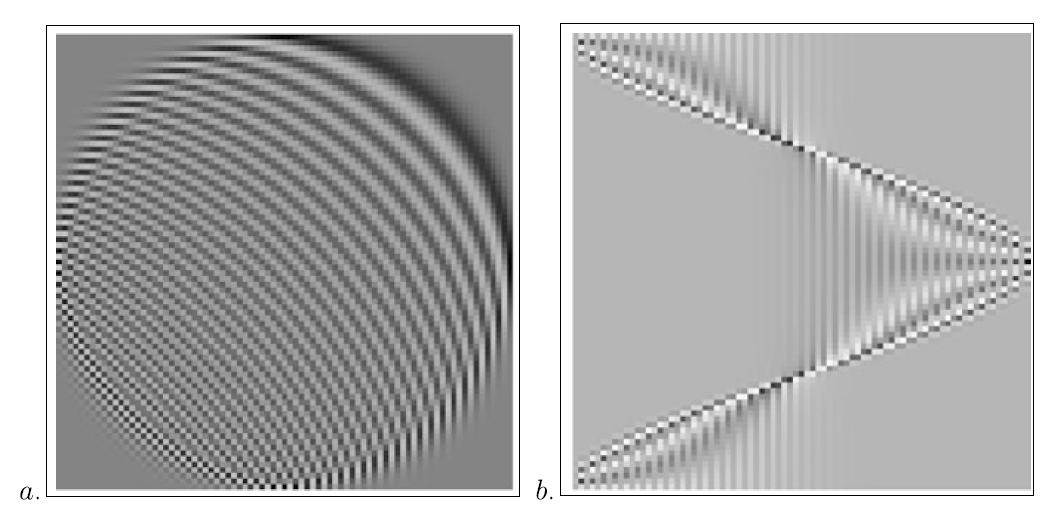
\includegraphics{images/img_13_1.png}
}
\caption{
\label{i13.1} \textbf{a.} Иллюстрация скалярного произведения $\langle m_3\mid m_1\rangle$; \textbf{b.} Изображение матрицы трансформации $\langle m_3\mid \sigma\rangle_{ont}$ (реальная часть). По горизонтали: $m_1$, по вертикали: $\sigma$}
\end {center}
\end {figure}


\end{document}